\documentclass{article}
\usepackage{graphicx}
\graphicspath{ {./images/} }
\usepackage[utf8]{inputenc}

\title{Assignment 25}
\author{Xiaoting Li (xil139) \\
Ziyu Zhang (ziz41) \\
Deniz Unal (des204)}
\date{March 2019}

\begin{document}

\maketitle

\noindent
\textbf{41. A problem $Y$ is NP-hard if there exists an NP-complete problem $X$ such that $X$ is polynomial-time reducible to $Y$ . Prove that the following problems are NP-hard. Keep your answers short.}\\ \newline
\textbf{(a) Prove that the subgraph-isomorphism problem defined in 34.5-1 is NP-hard by reduction from the CLIQUE problem defined earlier in chapter 34.}\\ \newline
Answer: To prove subgraph-isomorphism problem is NP-hard, we need to reduce CLIQUE to subgraph-isomorphism problem. Assume we have an instance of CLIQUE as $(G, k)$ in which there are $n$ vertices. We also have an instance of subgraph-isomorphism in which $G_1$ is a complete graph that has $k$ vertices and $G_2 = G$. It is easy for us to see that if there is a CLIQUE of size $k$ in $G$, we can find a solution to the subgraph-isomorphism by looking for the intersection between $k$ vertices in $G_1$ and $n$ vertices in $G_2$. If we have $k < n$, then this can be run in poly time. Since CLIQUE is NP-complete, so subgraph-isomorphism is NP-hard.\\ \newline
\textbf{(b) Prove that the integer programming problem defined in problem 34.5-3 is NP-hard by reduction from 3-CNF-SAT defined earlier in chapter 34.}\\ \newline
Answer: To prove the integer linear-programming problem, we need to reduce 3-CNF-SAT to the integer linear-programming problem. Let the variables in 3-CNF-SAT be $x_1, x_2, ... x_n$ and the let the variables in integer linear-programming problem be $s_1, s_2, ... s_3$. We restrict $s_1, s_2, ... s_n$ as $0 \leq s_i \leq T$, $T$ is an integer. We denote $0$ as false and any integer $> 0$ as true. For each clause ${x_1, x_2, x_3}$ in the 3-CNF-SAT problem, we have a constraint $s_1 + s_2 + s_3 \leq 0$. In order to have make each clause as true, we need to have at least one of the integer must be set larger than 0. Since 3-CNF-SAT is NP-hard, we can say that integer linear-programming is NP-hard. \\ \newline
\textbf{(c) Prove that the set partition problem defined in problem 34.5-5 is NP-hard by reduction from the SUBSET SUM problem defined earlier in chapter 34.} \\ \newline
Answer: To prove that the set partition problem is NP-hard, we need to reduce the SUBSET SUM problem to the set partition problem. Let's say we have set $S$ and the sum of all elements are $n$. We need to find the sum equals to $k$ in this set. And we have another set $S^{'} = S\cup (n-2k)$. Since $S^{'} = S\cup (n-2k)$, the sum of $S^{'}$ is $(2n-2k)$.  Since the sum of $S^{'}$ is $(2n-2k)$, we find set partition that has two subsets of $S^{'}$, each of which has the sum $(n-k)$. We know one of the set is $(n-2k)$, the other one is $k$. The one that is $k$ has the elements in $S$. In this way, we reduce SUBSET SUM to set partition. Since SUBSET SUM is NP-hard, so the set partition problem is NP-hard. \\ \newline
\textbf{(d) Prove that the longest-simple cycle problem defined in problem 34.5-7 is NP-hard by reduction from the Hamiltonian cycle problem defined earlier in chapter 34.} \\ \newline
Answer: To prove that the longest-simple cycle problem is NP-hard, we need to show that it is at least as hard as the Hamiltonian cycle problem. Let us have a graph G. We are trying to find out if it contains a Hamiltonian cycle. We complete the algorithm for finding a Hamiltonian cycle by making a call to an algorithm for the longest-simple cycle problem which decides whether the graph has a simple cycle of length at least the number of vertices in G. If we can have such an algorithm, we show that we also have an algorithm to solve Hamiltonian cycle problem. So, the longest simple cycle problem is at least as hard as the Hamiltonian cycle problem. \\ \newline 
\textbf{(e) Prove that the half-3-CNF problem defined in problem 34.5-8 is NP-hard by reduction from 3-CNF-SAT.} \\ \newline
Answer: Similar to the previous sub problem, to prove that half-3-CNF is NP-hard we need to show that solving that (new problem in our context) also means solving the 3-CNF-SAT problem (old hard problem in our context). We consider two 3-CNF formulas $\Phi$ and $\Phi'$ where $\Phi$ consists of m clauses and n variables and $\Phi'$ consists of $\Phi$ and m of some formulas (call them X) that are always satisfied, and 2m of some formulas (call them Y) that may or may not be satisfied. If we can have an assignment of the n variables that can satisfy $\Phi$ and an assignment of the variables that does not satisfy the 2m Y formulas , we would also have a satisfiable assignment for $\Phi'$ as 2m of its 4m clauses would always be satisfied (solution for half-3-CNF problem). But if we assume that there is no assignment of n variables that satisfies $\Phi$, If Y is not satisfied we will end up with m clauses satisfied in $\Phi'$ (Only X). If Y is satisfied than we will end up with 3m clauses satisfied in $\Phi'$ (X and Y). The number of satisfied clauses will be either strictly less or strictly more than the half of all clauses of $\Phi'$. So, if we  have a solution for the half-3-CNF problem, we would also have a solution 3-CNF-SAT problem which is NP-Complete. We showed that the half-3-CNF problem is at least as hard as the 3-CNF-SAT problem, so, we can say that half-3-CNF problem is NP-hard. \\ \newline
\textbf{42. Show that the 3-COLOR problem is NP-hard by reduction from the NP-complete 3-CNF-SAT problem. 3-COLOR is defined in problem 34-3 in the text, which also contains copious hints.}

\textbf As the problem 34-3, "To prove that 3-COLOR is NP-complete, we use a reduction from 3-CNF-SAT. Given a formula $\phi$ of m clauses on n variables x1 , x2 , . . . , xn , we construct a graph G = (V, E) as follows. The set V consists of a vertex for each variable, a vertex for the negation of each variable, 5 vertices for each clause, and 3 special vertices: TRUE , FALSE , and RED . The edges of the graph are of two types: ��literal�� edges that are independent of the clauses and ��clause�� edges that depend on the clauses. The literal edges form a triangle on the special vertices and also form a triangle on xi , not xi , and RED for i = 1, 2..., n." as shown in figure blow:
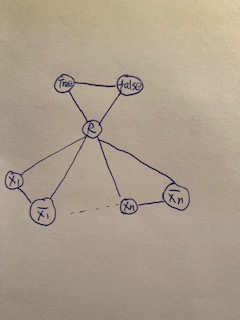
\includegraphics{image1.jpeg}
\\ \newline
(1) For the triangle with vertices xi, not xi, and Red, since there is already Red, so xi could be true, and not xi could be false, or xi could be false and not xi could be true. for any truth assignment for $\phi$, there is a 3-coloring of the graph containing just the literal edges (we could have xi be true and not xi be false or the other way around).
\\ \newline
(2) Here we agrue that if each of x, y, and z is colored c( TRUE ) or c( FALSE ), then the widget is 3-colorable if and only if at least one of x, y, or z is colored c( TRUE ). As shown in figure blow, if x, y, z all colored with false, then vertex A have to be false, and for the same reason, vertex B have to be false, which contradict with  vertex b is true.
\\ \newline
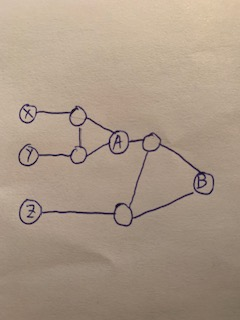
\includegraphics{image2.jpeg}
\\ \newline
Given the reason above, for any 3 cnf sat problem, we could use the strategy should above to create the reduction. From (1), we know that each of the variable must be true or false, and its negation must be false or true accordingly, from (2) we know that each of the clause will only be true if we assign one of x, y, z to be true, which means making one of the according clause to be true. Since 3 cnf sat is NP-complete and we found a poly-time way to reduce 3 cnf sat to 3 color, so 3 color is NP-hard.
\end{document}
